% \documentclass[screen, , oneside, authorversion,nonacm,authoraddress=false, margin=1in]{acmart}
% ^^^ use this for the original format


% vvv use this for the actual submission

\documentclass[sigconf, screen, authorversion, authoraddress=false, oneside]{acmart}

%fixes every other page indent issues, modify margins as needed
% \setlength{\oddsidemargin}{-0.18in}
% \setlength{\evensidemargin}{-0.18in}

\usepackage{cite}
\usepackage{multirow}
\usepackage{caption}
\usepackage{graphicx}
\usepackage{wrapfig}
\usepackage{makecell}
\usepackage{hyperref}
\usepackage{subcaption}
\usepackage{float}

\renewcommand{\thesubfigure}{\Alph{subfigure}}

%necessary package to include bibliography in references
\usepackage[backend=biber, style=acmnumeric]{biblatex}
\addbibresource{refs.bib}
\bibliography{refs}




\begin{document}

%%
%% The "title" command has an optional parameter,
%% allowing the author to define a "short title" to be used in page headers.
\title{Double Insertion Mutation Hydrogen Proximity Analysis}

\author{James Tessmer}
\email{tessmej@wwu.edu}
\affiliation{
  \institution{Western Washington University}
  \city{Bellingham}
  \state{Washington}
  \country{USA}
}
\author{Boris Weinfurt}
\email{weinfub@wwu.edu}
\affiliation{
  \institution{Western Washington University}
  \city{Bellingham}
  \state{Washington}
  \country{USA}
}
\author{Takira Boltman}
\email{boltmat@wwu.edu}
\affiliation{
  \institution{Western Washington University}
  \city{Bellingham}
  \state{Washington}
  \country{USA}
}
\author{Andrew Downing}
\email{downina3@wwu.edu}
\affiliation{
  \institution{Western Washington University}
  \city{Bellingham}
  \state{Washington}
  \country{USA}
}
\author{Caroline Kays}
\email{kaysc@wwu.edu}
\affiliation{
  \institution{Western Washington University}
  \city{Bellingham}
  \state{Washington}
  \country{USA}
}
\author{Colton Ferriole}
\email{ferrioc@wwu.edu}
\affiliation{
  \institution{Western Washington University}
  \city{Bellingham}
  \state{Washington}
  \country{USA}
}

\begin{abstract}
The stability and functionality of proteins are critically influenced by structural changes induced by mutations. This study investigates the effects of double insertion mutations on hydrogen bonds, focusing on their proximity to the mutation sites. Using computational methods, we analyzed 4 protein structures (1crn, 1csp, 1hhp, 1cdz) and evaluated hydrogen bond alterations induced by outlier mutations. Through an automated data processing pipeline, we determined the distances between insertion sites and hydrogen bonds, revealing patterns in how certain amino acids influence the structure.
\end{abstract}

\maketitle

\keywords{Protein mutations, 
Double insertion mutation,
Hydrogen bond analysis, Protein stability, Computational biology, Alpha helices, Beta sheets, Structural bioinformatics, Rosetta software, HBPLUS,
Protein data bank (PDB), Amino acid insertion, Protein folding, Structural flexibility, Hydrophobic and hydrophilic interactions}



\section{Introduction}
Double-insertion mutations can have a profound impact on protein structure and function, influencing both stability and flexibility. These mutations introduce additional amino acids that may disrupt critical interactions within the protein, leading to conformational changes. Such alterations can destabilize the protein or modify its dynamics, potentially impairing its biological function. Examining the effects of double-insertion mutations provides insights into the structural basis of these changes. This analysis is particularly relevant for understanding disease-associated variants where structural disruptions play a key role.

\begin{figure}[ht]
    \centering
    % 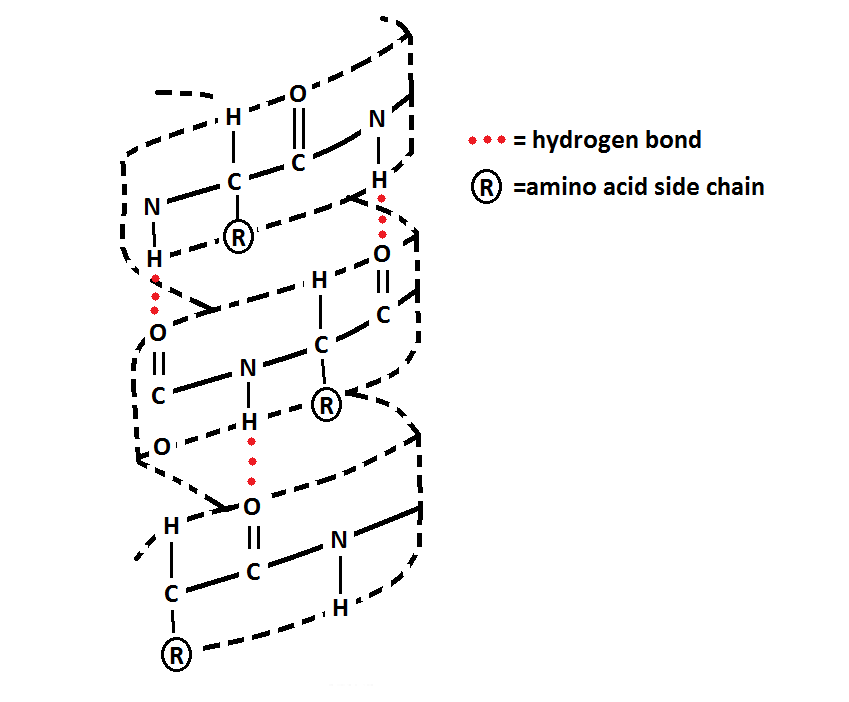
\includegraphics[width=0.4\textwidth]{hydrogen_structure.png}
    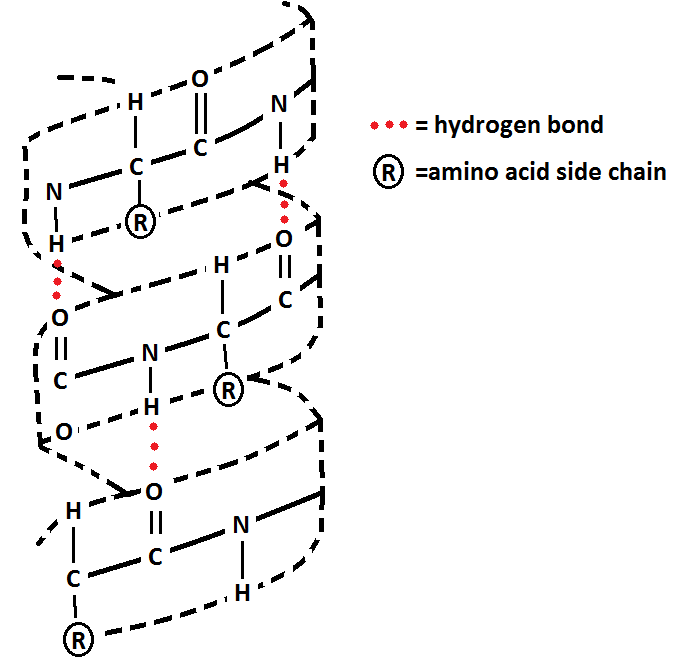
\includegraphics[width=0.4\textwidth]{hbond_structure_crop.png} %retains more detail
    \caption{2D representation of the structure of a typical alpha-helix. Figure from Ben Russell's Thesis on Protein Encapsulated Gold Nanoclusters for Biological Applications \cite{phdthesis}.}
    \Description{"2D representation of the structure of a typical alpha-helix. While hydrogen bonding is relatively weak, the amount of hydrogen bonding taking place along the coil offers enough strength for the secondary structure to keep its shape Figure from Ben Russell's Thesis". Found on page 71.\cite{phdthesis}.}
    % \label{Figure 1}
    \label{fig:Figure1}
\end{figure}

As shown in \hyperref[fig:Figure1]{Figure 1}, hydrogen bonds \cite{ArunanDesirajuKleinSadlejScheinerAlkortaClaryCrabtreeDannenbergHobzaKjaergaardLegonMennucciNesbitt+2011+1619+1636} offer strength to the secondary structure. Changes to these hydrogen bonds can impact the stability and conformation of the structure. This project focuses on examining the effects of double-insertion mutations on hydrogen bonds. By analyzing the existing datasets of protein mutants (1crn, 1csp, 1hhp, and 1cdz), we aim to identify which trends among outlier mutations cause the most impact on the resulting hydrogen bonds, and how different mutations affect the proximity of the hydrogen bonds to the mutation site.



%made a comment as the first 1-2 sentences of motivation could
%be re-worded to be clearer
\section{Motivation}
Understanding the effects of mutations on the formation of hydrogen bonds can provide insight into the effect of that mutation. Mutations can disrupt or displace hydrogen bonds, causing changes in stability or rigidity of the protein. Particularly when the insertion or deletion can affect hydrogen bonds farther away from the mutation sites. When a protein undergoes mutation, several factors can be analyzed to assess the mutation’s impact, one of which is the pattern of hydrogen bonds. These bonds are critical in forming and stabilizing protein folds \cite{BORDO1994504}. Additionally, identifying which trends among insertions cause hydrogen bonds to shift closer or further from the insertion site can reveal how these insertions affect the protein's structure. Analyzing these trends across multiple proteins may offer broader insights into which mutations are likely to impact protein function. Ultimately, this knowledge could be applied towards therapeutic methods to treat or prevent disease causing proteins.

%--------------------------------------------related works------------------------------------------------

\begin{figure*}[!ht]
    \centering
    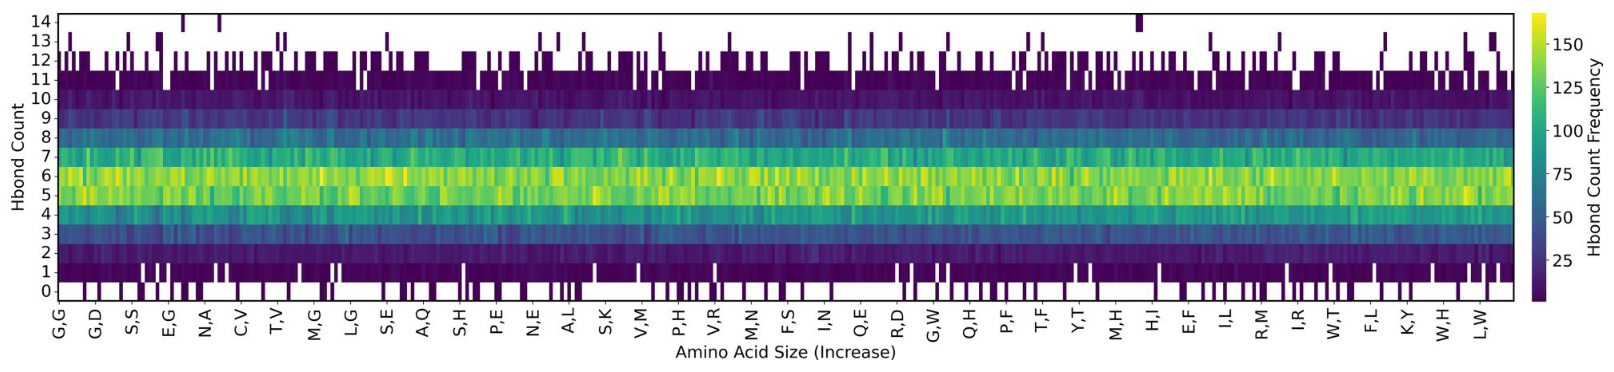
\includegraphics[width=0.975\textwidth]{multimute_hbond_plot.png}
    \caption{From Li \textit{et al.}, [2024] \cite{10.1093/bioadv/vbae138}. Count of hydrogen bonds for insertion pairs, ordered from the smallest pairs to largest.}
    %I feel like we should make an explicit mention that this figure is from Changrui/Filips paper..
    \Description{A graph showing hydrogen bond counts increasing with larger amino acid sizes.}
    \label{Figure 2}
\end{figure*}

\section{Related Work}
We are continuing the previous work done by Li \textit{et al.}, [2024] of studying how pairs of mutations impact protein structure \cite{ArunanDesirajuKleinSadlejScheinerAlkortaClaryCrabtreeDannenbergHobzaKjaergaardLegonMennucciNesbitt+2011+1619+1636}. The goal of this study was to understand how specific changes, such as inserting pairs of amino acids, affect protein stability (such as with hydrogen bond count in \hyperref[fig:Figure2]{Figure 2}) and structure. This is especially important research for those in the medical field whose expertise lies in targeting diseases that are caused by protein mutations, such as Alzheimer’s and Cystic Fibrosis. Their research was done in silico using PDB files and simulating the double insertion of amino acids using Rosetta, which avoided the time and cost requirements of performing experiments in a physical lab. The Rosetta software involved procedures such as inverse kinematics, as well as Remodel and Loop protocols to observe changes to a protein’s structure.  

To categorize findings, mutations were grouped into pairs based on insertion into alpha helices, a critical structure to the protein. Amino acids were then analyzed by natural volume, being further categorized by their given size. Their research led them to the conclusion that larger amino acids, such as tryptophan, disrupted protein structures significantly versus smaller amino acids, such as alanine or glycine. They also found that inserting mutations into protein structures, such as alpha helices, can impact stability differently. Mutations around non-active sites, or less integral structures, showed more flexibility and stability. While their research remains inconclusive, the authors suggest that looking into hydrophilic and hydrophobic amino acids and the integrity of the structure upon insertion of these might bring forth more conclusions, as well as using machine learning to analyze large datasets for other patterns. Furthermore, the authors also suggest using contact maps to analyze how amino acids interact with each other to better predict the integrity of the structure with specific pairs of mutations.

%------------------------------------------Methods--------------------------------------------------

\section{Methods}

To analyze the impacts of double insertions and their respective hydrogen bond formations on protein structures, we began by processing raw data. The original JSON files obtained from Rosetta for each protein were parsed into PDB files, which were then analyzed using HBPLUS \cite{HBPLUS_tool}. HBPLUS specializes in generating hydrogen bond information from a given PDB file.
\\
Using the updated PDB file and the HB2 file output from HBPLUS, we identified specific atoms based on residue numbers and atom names, uniquely identifying their x, y, z coordinates. Hydrogen bond positions were determined by calculating the midpoint between the donor and acceptor atoms identified by HBPLUS. The insertion locations were defined by the coordinates of their CA atoms. The distances between each insertion point and the hydrogen bond midpoints were calculated, with the closer of the two distances being recorded as the final result for each hydrogen bond.
\\
To further refine the dataset, we applied the following filtering criteria:
\begin{enumerate}
    \item \textbf{Outlier Selection}: Mutations with fewer than two standard deviations from the mean for average distance were filtered out to account for outliers.
    \item \textbf{Proximity Filtering}: Mutations where both insertion points were within 10\% of the protein's total length were excluded to avoid confounding effects due to proximity rather than genuine impacts on hydrogen bond formation.
\end{enumerate}

\begin{figure}
    \centering
    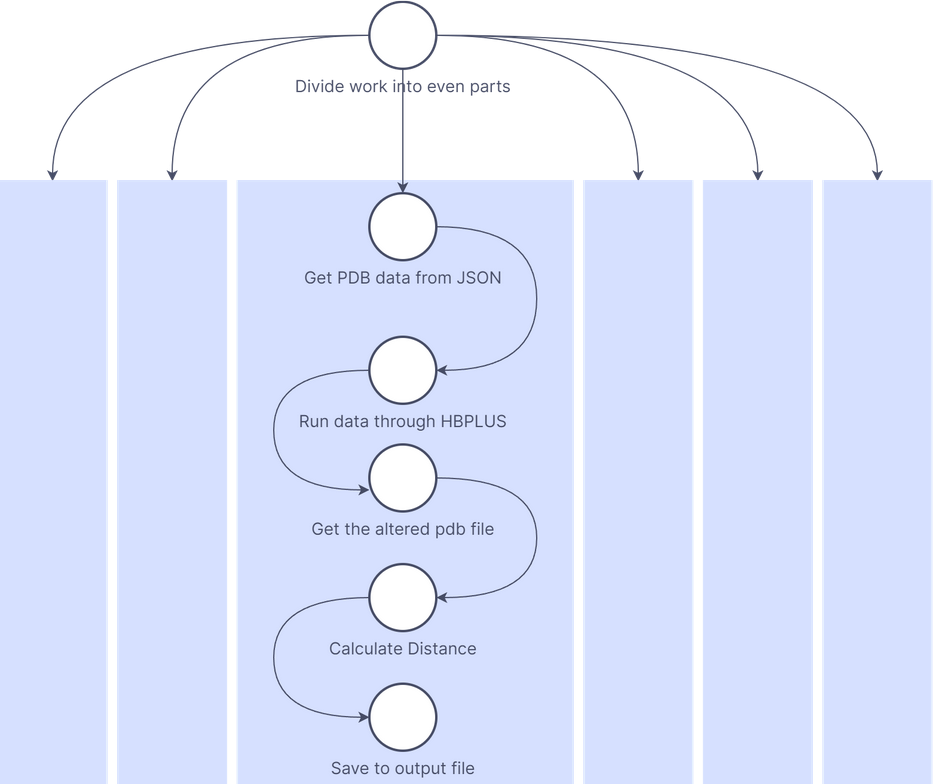
\includegraphics[width=0.4\textwidth]{double_ins_method.png}
    \caption{A visual illustration of the methods used to collect the data.}
    \label{fig:Figure3}
    \Description{Visualization showing how the data was parsed through different tools that could then be used for analysis.}
\end{figure}
Following refinement, the remaining mutations were sorted by hydrogen bond count, from lowest to highest. For each protein, the subset was further reduced to the top 10 mutants with the lowest hydrogen bond counts. This yielded a final table for each protein, highlighting mutants with significantly higher average distances, while controlling for confounding variables like proximity of insertion locations. These mutants were identified as having a potential reduction in the number of hydrogen bonds local to the insertion sites. \hyperref[fig:Figure3]{Figure 3} illustrates our processes in parsing, collecting, and then analyzing the data.

%------ I put the figure down at the end of the document
% \hyperref[fig:Figure]{}
% \begin{figure}
%     \centering
%     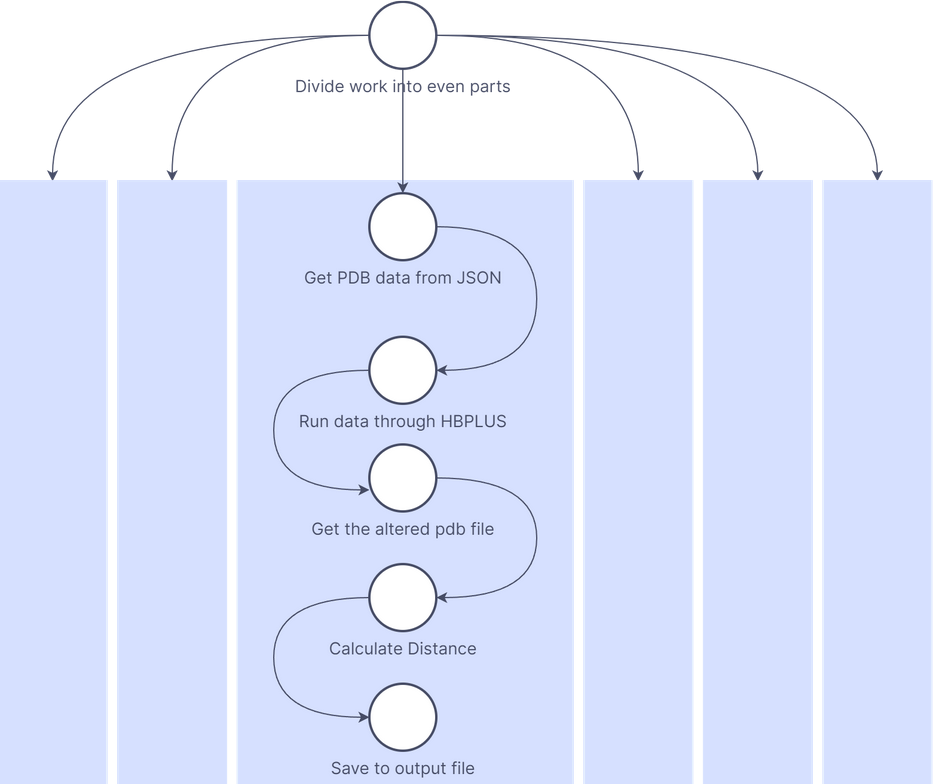
\includegraphics[width=0.4\textwidth]{double_ins_method.png}
%     \caption{Figure 6}
%     \label{fig:Figure6}
% \end{figure}

%----------------------------------------Results----------------------------------------------------


\section{Results}
These results are based off of very large data sets, the smallest of which, 1crn, contained roughly 400,000 mutants. We are confident that the size of our datasets allows our findings to be generalizable to other mutant proteins. In fact, we report observed trends across all proteins analyzed, whose generalization is supported by the dataset of millions of mutants.


\subsection{1hhp}
\begin{figure}[!ht]
    \centering
    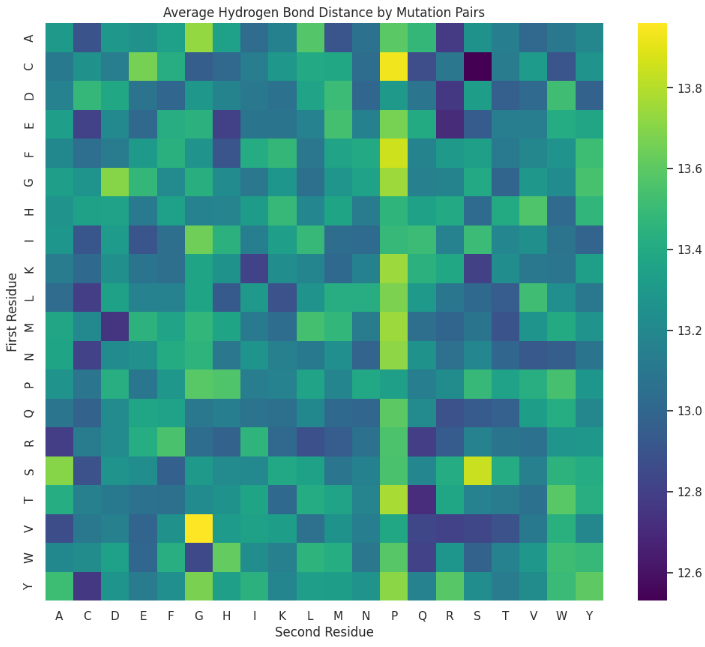
\includegraphics[width=0.46\textwidth]{residue_to_distance.png} 
    \caption{2D heatmap of average hydrogen bond distance by mutation pair 
 for 1HHP}
    \Description{2D Heatmap of the average hydrogen bond distances by first and second insertions (of amino acids)}
    \label{fig:Figure4}
\end{figure}



Certain amino acids were more likely to have a higher average distance to hydrogen bonds than others, such as the 1hhp residue mappings in \hyperref[fig:Figure4]{Figure 4}. Most combinations in which proline is the second amino acid inserted appear to result in a higher average, compared to other pairs of insertions, distance from insertion to the hydrogen bond. This is particularly noticeable for the pairing of cysteine and proline. This pattern does not seem to hold for cases where proline is inserted as the first amino acid. Other seeming outliers are the pairing of V-G and S-S. These patterns do not hold for the top 10 outliers for 1hhp (\hyperref[table:1]{Table 1}). 


\begin{figure}[ht]
    \centering
    % 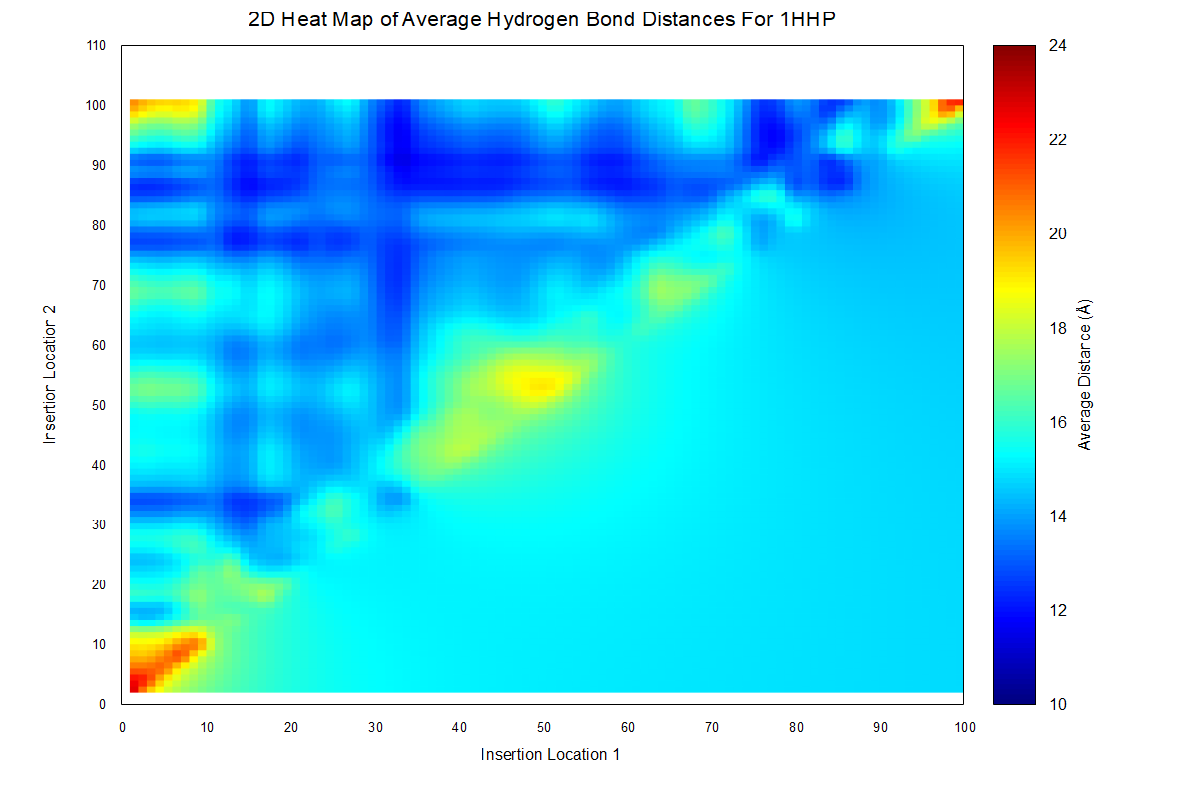
\includegraphics[width=0.5\textwidth]{heatmap_1hhp_all.png} 
    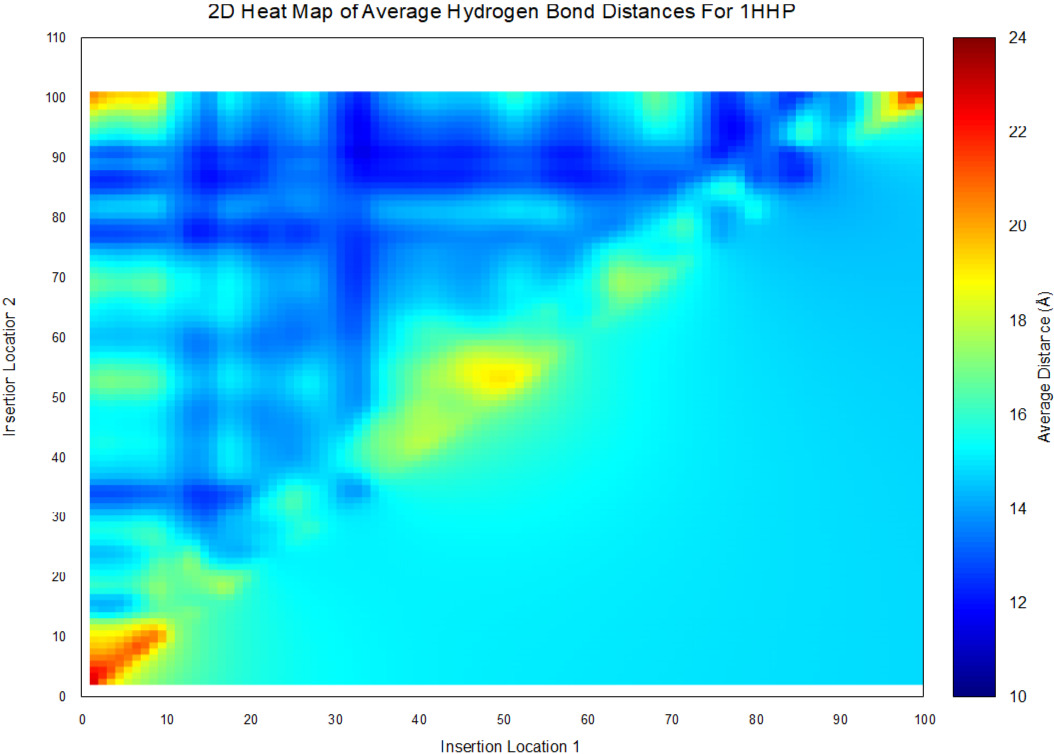
\includegraphics[width=0.5\textwidth]{heatmap_1hhp_all_recrop.jpeg} 
    \caption{2D heatmap of average hydrogen bond distance by insertion location for 1HHP}
    \label{fig:Figure5}
\end{figure}

\begin{table}[!ht] %][h!] or [ht] ?
    \centering
    \refstepcounter{table}
    \textbf{\large Table \thetable: 1hhp outliers} \\[1ex]
    {\small
    \setlength{\tabcolsep}{2pt} % Adjust the column spacing
    \begin{tabular}{cccccccc}
    \toprule
    \makecell{Ins.\\Loc. 1} & 
    \makecell{Residue\\1} & 
    \makecell{Ins.\\Loc. 2} & 
    \makecell{Residue\\2} & 
    \makecell{Avg.\\Dist.} & 
    \makecell{Total\\Bonds} & 
    \makecell{SD Avg.\\Dist.} & 
    \makecell{SD HBond\\Count} \\
    \midrule
    74 & L & 85 & H & 25.80 & 31 & 4.20 & -4.24 \\
    74 & V & 85 & K & 25.35 & 32 & 4.04 & -4.08 \\
    74 & N & 87 & L & 25.90 & 32 & 4.24 & -4.08 \\
    74 & S & 85 & S & 25.81 & 32 & 4.21 & -4.08 \\
    73 & L & 84 & F & 25.74 & 33 & 4.18 & -3.92 \\
    73 & E & 84 & Q & 25.50 & 33 & 4.09 & -3.92 \\
    74 & V & 85 & V & 25.84 & 34 & 4.22 & -3.77 \\
    73 & I & 84 & V & 25.48 & 34 & 4.09 & -3.77 \\
    73 & H & 84 & L & 26.25 & 34 & 4.37 & -3.77 \\
    73 & R & 85 & C & 25.45 & 35 & 4.08 & -3.61 \\
    \bottomrule
    \end{tabular}
    }
    \caption*{Table 1: Top 10 outliers for 1hhp based on (lowest) hydrogen bond count after filtering to account for proximity and to only show statistically significant outliers based on average distance.}
    \label{table:1}
\end{table}

These outliers have consistent first and second insertion locations with only a tiny spread, but this consistency is not seen in which amino acids are present in the outlier mutants. The first insertion location in these mutants is seen to always be residue 73 or 74 while the second location varies between residues 84, 85, and 87 with most being the former 2 residues. Both of these location clusters fall within two different beta sheets, and this combination of regions is usually seen to have much lower average distances (14-15 Å) (\hyperref[fig:Figure5]{Figure 5}).
\subsection{1csp}


\begin{table}[!ht] %][h!] or [ht] ?
    \centering
    \refstepcounter{table}
    \textbf{\large Table \thetable: 1csp outliers} \\[1ex]
    {\small
    \setlength{\tabcolsep}{2pt} % Adjust the column spacing
    \begin{tabular}{cccccccc}
    
    \toprule
    \makecell{Ins.\\Loc. 1} & 
    \makecell{Residue\\1} & 
    \makecell{Ins.\\Loc. 2} & 
    \makecell{Residue\\2} & 
    \makecell{Avg.\\Dist.} & 
    \makecell{Total\\Bonds} & 
    \makecell{SD Avg.\\Dist.} & 
    \makecell{SD HBond\\Count} \\
    \midrule
    35 & C & 48 & G & 24.56 & 19 & 4.87 & -3.48 \\
    49 & M & 61 & E & 23.89 & 19 & 4.60 & -3.48 \\
    49 & D & 62 & I & 24.89 & 20 & 5.01 & -3.27 \\
    50 & S & 62 & K & 22.53 & 20 & 4.05 & -3.27 \\
    50 & S & 62 & G & 25.47 & 20 & 5.25 & -3.27 \\
    50 & I & 62 & F & 25.42 & 20 & 5.23 & -3.27 \\
    50 & F & 62 & R & 23.26 & 20 & 4.35 & -3.27 \\
    49 & Y & 62 & A & 23.21 & 20 & 4.33 & -3.27 \\
    48 & L & 61 & Q & 24.42 & 20 & 4.82 & -3.27 \\
    49 & C & 62 & C & 24.68 & 20 & 4.93 & -3.27 \\
    \bottomrule
    \end{tabular}
    }
    \caption*{Table 2: Top 10 outliers for 1csp based on (lowest) hydrogen bond count after filtering to account for proximity and to only show statistically significant outliers based on average distance.}
    \label{table:2}
\end{table} 


Similarly to 1hhp, the top 10 outliers for 1csp (\hyperref[table:2]{Table 2}) tend to cluster around specific insertion locations with the same lack of consistency in amino acids. The one exception to this is the top outlier which is found with the first insertion at residue 35 and the second at residue 48 versus the other mutants with the first insertion found around residues 48 to 50 and the second found around residues 61 or 62. Residue 35 is found in an outer loop of the protein and not particularly close to any substructure, while residue 48 is in a beta sheet. Residues 48 to 50 are all in that same beta sheet. Residue 61 is the final residue of a beta sheet, and residue 62 is directly adjacent. These two regions are both beta strands in the same beta sheet and are only 5 Å apart from each other. This region of the protein showed middling average distance across all mutants (around 14 Å) compared to the outliers (around 24 Å) which show a roughly 70\% increase in average distance. All outliers show both significantly higher than the mean average distance and significantly lower than the mean hydrogen bond count. The properties of inserted amino acids are exactly evenly split on hydrophobic and hydrophilic.
\subsection{1crn}

\begin{table}[!ht] %Refers to Table 3, T10 outliers for 1crn
    \centering
    \refstepcounter{table}
    \textbf{\large Table \thetable: 1crn outliers} \\[1ex]
    {\small
    \setlength{\tabcolsep}{2pt} % Adjust the column spacing
    \begin{tabular}{cccccccc}
    \toprule
    \makecell{Ins.\\Loc. 1} & 
    \makecell{Residue\\1} & 
    \makecell{Ins.\\Loc. 2} & 
    \makecell{Residue\\2} & 
    \makecell{Avg.\\Dist.} & 
    \makecell{Total\\Bonds} & 
    \makecell{SD Avg.\\Dist.} & 
    \makecell{SD HBond\\Count} \\
    \midrule
    36 & W & 48 & S & 20.09 & 26 & 4.11 & -1.89 \\
    2 & K & 38 & M & 20.27 & 26 & 4.18 & -1.89 \\
    3 & G & 48 & S & 21.06 & 26 & 4.52 & -1.89 \\
    35 & R & 41 & Y & 20.95 & 27 & 4.47 & -1.60 \\
    35 & M & 40 & I & 19.93 & 27 & 4.04 & -1.60 \\
    2 & R & 48 & R & 19.91 & 27 & 4.03 & -1.60 \\
    1 & P & 39 & C & 20.23 & 27 & 4.17 & -1.60 \\
    1 & T & 39 & P & 21.18 & 27 & 4.57 & -1.60 \\
    1 & I & 37 & S & 21.19 & 27 & 4.57 & -1.60 \\
    35 & W & 42 & Q & 20.05 & 28 & 4.09 & -1.31 \\
    \bottomrule
    \end{tabular}
    }
    \caption*{Table 3: Top 10 outliers for 1crn based on (lowest) hydrogen bond count after filtering to account for proximity and to only show statistically significant outliers based on average distance.}
    \label{table:3}
\end{table}

The top outliers for 1crn (\hyperref[table:3]{Table 3}) fall into two distinct regions, with the first region having the first insertion at residues 35 or 36 and the second being spread around 40 to 42 with one instance of residue 48. The second region has the first insertion in the range of residues 1 to 3 and the second insertion around residues 37 to 39 with two instances of residue 48. This is a higher spread in location than the other proteins, but there are still two distinct clusters. The first cluster has insertion 1 at the tail end of a beta sheet and insertion 2 in a loop that is not close to any substructure. Cluster 2 has insertion 1 at the very start of a beta sheet, and insertion 2 is the same as cluster 1. While the residue number of the first insertion locations are far apart, these two groups of residues are only 6 Å apart. 1crn also has 2 alpha helices in close proximity which are at the far end of where all these insertion location clusters are. The notable exception is the three instances of residue 48 which is the last residue of the protein. Due to the protein's structure, this residue is only 6 Å away from the first alpha-helix while the other second insertion sites are closer to 14 Å away. Note that while all mutants have an average hydrogen bond distance that is significantly higher than the mean for 1crn, none of them have a significantly lower number of hydrogen bonds.
\subsection{1cdz}
\begin{table}[!ht] %Table 4, T10 outliers for 1cdz
    \centering
    \refstepcounter{table}
    \textbf{\large Table \thetable: 1cdz outliers} \\[1ex]
    {\small
    \setlength{\tabcolsep}{2pt} % Adjust the column spacing
    \begin{tabular}{cccccccc}
    \toprule
    \makecell{Ins.\\Loc. 1} & 
    \makecell{Residue\\1} & 
    \makecell{Ins.\\Loc. 2} & 
    \makecell{Residue\\2} & 
    \makecell{Avg.\\Dist.} & 
    \makecell{Total\\Bonds} & 
    \makecell{SD Avg.\\Dist.} & 
    \makecell{SD HBond\\Count} \\
    \midrule
    49 & P & 59 & P & 28.49 & 54 & 5.62 & -3.10 \\
    49 & D & 59 & N & 31.36 & 54 & 6.75 & -3.10 \\
    48 & L & 58 & Y & 28.24 & 55 & 5.53 & -2.90 \\
    48 & V & 59 & P & 24.96 & 55 & 4.24 & -2.90 \\
    47 & M & 57 & K & 24.44 & 55 & 4.04 & -2.90 \\
    47 & P & 59 & H & 28.73 & 55 & 5.72 & -2.90 \\
    47 & D & 59 & H & 29.06 & 55 & 5.85 & -2.90 \\
    48 & M & 59 & L & 25.07 & 55 & 4.28 & -2.90 \\
    48 & E & 58 & R & 26.08 & 55 & 4.68 & -2.90 \\
    47 & Y & 58 & G & 28.04 & 56 & 5.45 & -2.70 \\
    \bottomrule
    \end{tabular}
    }
    \caption*{Table 4: Top 10 outliers for 1cdz based on (lowest) hydrogen bond count after filtering to account for proximity and to only show statistically significant outliers based on average distance.}
    \label{table:4}
\end{table}

As with previous proteins, the top outliers for 1cdz (\hyperref[table:4]{Table 4}) shows clustered insertion locations. Insertion location 1 for outliers can be found in residues 47 to 49 and insertion location 2 can be found in residues 57 to 59. The region of insertion location 1 falls in the middle of a beta sheet which is itself in almost the center, spatially, of the protein. The region of insertion location 2 falls into the center of an alpha-helix. 1cdz has 4 alpha helices, with 3 being on the opposite end of the protein from the one containing insertion location 2. This combination of regions, across all mutants for the protein, has an average distance to hydrogen bonds of around 15 Å (\hyperref[fig:Figure6]{Figure 6}) while the outliers have an average closer to 27 Å which is an increase of roughly 80\%. The consistency of which amino acids are represented is, again, low. All 10 mutants also show at least 4 standard deviations away from the mean for average hydrogen bond distance, and a significantly lower number of hydrogen bonds than the average.

\begin{figure}[ht]
    \centering
    % 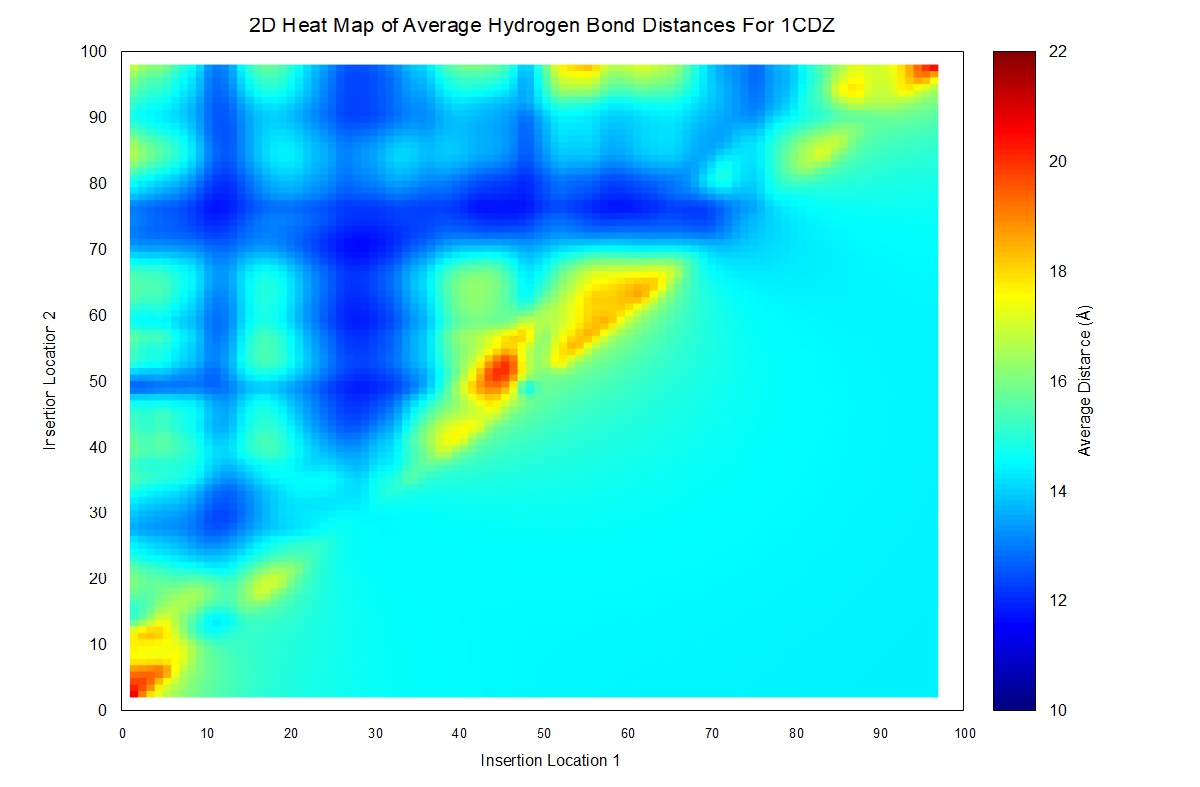
\includegraphics[width=0.5\textwidth]{heatmap_1cdz_all.png} 
    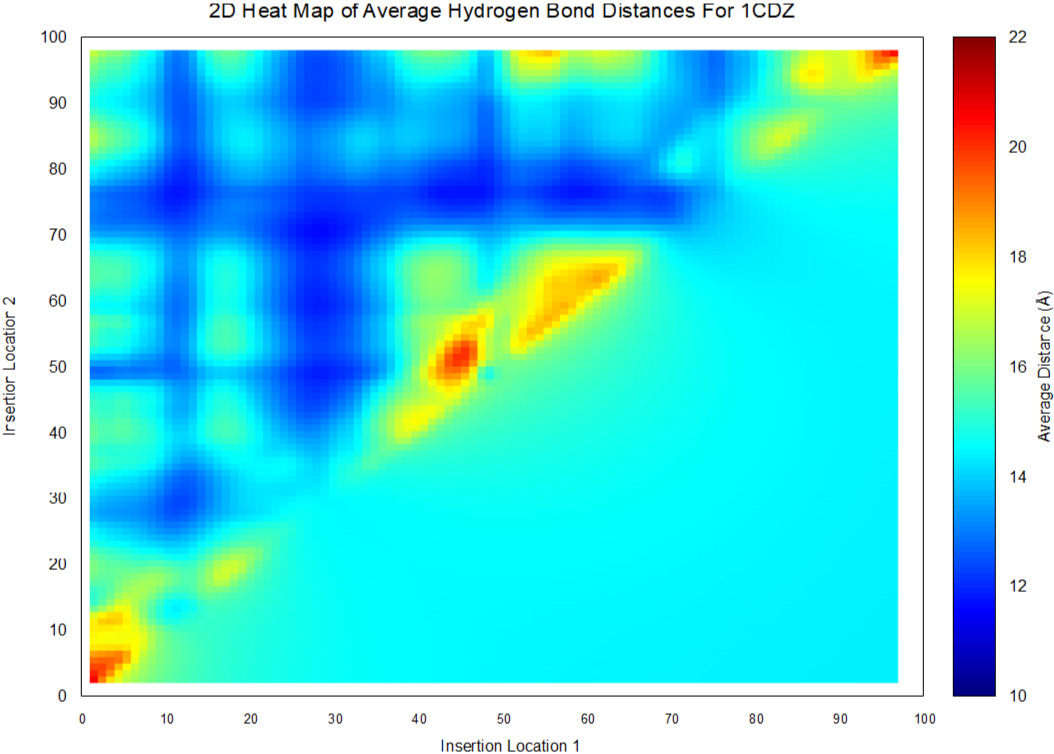
\includegraphics[width=0.5\textwidth]{heatmap_1cdz_all_recrop.jpeg} 
    \caption{2D heatmap of average hydrogen bond distance by insertion location for 1CDZ}
    \label{fig:Figure6}
\end{figure}


\subsection{Cross Protein trends}
There are some patterns that appear across all proteins. The first is that top outliers tend to cluster around the same 3D-space locations. Some of these insertion locations might not be near each other in sequence (such as the insertion location 1 of 1crn), but they tend to be only a few Angstroms away from each other in real space. The second trend observed is that outliers in all proteins tend to have at least one insertion into either an alpha-helix or beta sheet. The last trend seen is an almost even spread of what amino acids are present in the top outliers. There is some skew present, but it is not significant enough to say any amino acid is overly represented in outliers across proteins. There is also at least one instance of all 20 naturally occurring amino acids.


\section{Discussion}
The averages for 1hhp shows that proline seems to be correlated with a higher than average distance to hydrogen bonds. It is possible that this trend is due to the hydrophobic properties of proline. It does not frequently participate in hydrogen bonding, so it would likely not have any hydrogen bonds itself. Its large hydrophobic side chain may also influence local residues to not hydrogen bond as well. However, proline was not represented at all in the top 10 outliers for 1hhp. This shows that trends seen in averages for mutants do not correlate well to outliers. Furthermore, we saw that there was no clear trend at all in which amino acids were present in outliers. this indicates that the residue inserted is a poor metric for determining the impact on local hydrogen bonds.

In contrast, the location of insertion seems to correlate well to how a specific mutation will impact bonds. The fact that outliers tend to cluster into specific regions of the protein indicates that something about those regions makes the present hydrogen bonds susceptible to disruption, leading to local bonds either being unable to form or shifting further away. Many of the possible characteristics of these regions leading to this trend are unclear, however the presence or adjacency to a substructure does appear to be an important factor. Nearly all outliers were present in either a beta sheet or alpha-helix. This fact fits, as substructures of proteins tend to be richer in hydrogen bonds than unstructured loops. The lower count of bonds indicate that this hydrogen bond rich regions are being disrupted.

Indeed, this correlation of lower hydrogen bond count and higher distance does indicate that these specific outliers have appeared because they are disrupting local bonds. We are not sure what it is that is about these outliers that is causing this possible disruption. All amino acids are represented in the outliers, so it could be more likely that some of these regions are sensitive enough to change that any insertion at all would cause major disruption. However, as discussed the outliers are in the same regions that most mutations have middling average distance, so clearly not all mutations to these locations are as impactful.

These trends could be influenced by other trends within the protein. As previously stated, many outliers were present in substructures which is not a coincidence. Alpha helices, and to a lesser extent beta sheets, are far more rich in hydrogen bonds than unstructured loops. Further, the tertiary structure of the target protein could have alpha helices and beta sheets in close proximity or further apart. As seen in 1cdz, there is a lone alpha-helix as far away as possible from the other 3 helices clustered together. Our 1cdz mutants showed fewer bonds and higher average distance with an insertion into this alpha-helix, but that does imply mean it had a greater impact than another mutant with insertions into the 3 clustered helices. It could be that, simply due to the conformation of the protein, a mutant that highly impacted local bonds didn't have a significantly higher average distance. Trends like these, hydrogen bond rich regions and their proximity to each other, should be considered when determining impact. Our approach did not account for all of these possible trends so we may have left some impactful mutants unaccounted for, but we are confident the outliers we did present are representative samples of high impact mutants.

It is worth noting that we are unable to make some claims. Our data filtering for outliers attempts to account for instances where insertions being close together could lead to higher average distance. It also attempts to account for instances where relative location plays a factor by sorting mutants by number of bonds, as it's unlikely a mutant with a high average distance due to simple being far away from hydrogen bond rich regions would also have significantly fewer hydrogen bonds. Our outliers for 1crn did not show significantly fewer bonds, and are located, for the most part, as far away from alpha helices as they can be. This could mean that our filtering did not fully remove outliers due to the above factors, or they could truly be impacting local bonds. We also did not track which bonds stayed intact and which bonds shifted or were missing, so we cannot claim exactly which bonds are being affected or how. Additionally, we are lacking measurements on which bonds in each mutant are specifically 'far' (and as defined previously) versus 'close'.

Overall, it can be seen that our work to uncover how insertions affect hydrogen bonds has revealed a couple of key things. To summarize, the first is that the specific amino acid inserted does not seem to correlate with whether or not a mutation will have a large impact on local hydrogen bonds. A better metric to determine this is the location of insertions, particularly if they are in a substructure such as a beta sheet. Lastly, trends that emerge in the average of all mutants are not reflective of what mutants will be outliers. Outliers were frequently found in locations that trends implied they wouldn't, and trends in amino acids overall were not present in outliers.

\section{Future Work}

\subsection{Missing Protein Mutants}
Our dataset comes from Li \textit{et al.}, [2024] \cite{10.1093/bioadv/vbae138} which was unable to generate every possible mutant. Although there are enough mutants to be analyzed to be confident in our claims, it could be worthwhile to investigate why Rosetta was unable to generate some mutants. There could be a shared factor that is relevant to the biology of these mutants, or it could be a computational limitation.

\subsection{Hydrogen Bond Localization Analysis}
One potential area for future analysis involves investigating the localization of hydrogen bonds in wild-type versus mutated proteins for the locations of inserted (or wild-type) residues. This analysis could help identify whether hydrogen bonds form in the same regions or whether their positions shift when different amino acids are inserted. Such insights would provide a deeper understanding of how mutations impact the stability and structure of the protein at the atomic level.

\subsection{Rigorous Statistical Analysis}
While this study has produced preliminary results, a more rigorous statistical analysis of the data is needed. In particular, performing statistical tests would allow us to definitively determine if certain values are outliers or significantly different from other values. Such analyses would improve the robustness and reliability of the conclusions drawn from the dataset.

\subsection{More Exhaustive Data Collection}
Our methods included only one measurement per hydrogen bond. Future work could benefit from collecting the distance from each bond to both insertion points. Additionally collecting and considering data such as the properties of amino acids surrounding insertion locations could provide more concrete insight into why outliers have a greater distance or fewer bonds. It could also help eliminate confounding variables that we had trouble dealing with such as whether proximity of insertion locations and relative location of insertions to substructures.



\printbibliography



\end{document}
